\documentclass[12pt, titlepage]{article}

\usepackage{fullpage}
\usepackage[round]{natbib}
\usepackage{multirow}
\usepackage{booktabs}
\usepackage{tabularx}
\usepackage{graphicx}
\usepackage{float}
\usepackage{hyperref}
\usepackage{ulem}
\hypersetup{
    colorlinks,
    citecolor=blue,
    filecolor=black,
    linkcolor=red,
    urlcolor=blue
}

%% Comments

\usepackage{color}

\newif\ifcomments\commentstrue %displays comments
%\newif\ifcomments\commentsfalse %so that comments do not display

\ifcomments
\newcommand{\authornote}[3]{\textcolor{#1}{[#3 ---#2]}}
\newcommand{\todo}[1]{\textcolor{red}{[TODO: #1]}}
\else
\newcommand{\authornote}[3]{}
\newcommand{\todo}[1]{}
\fi

\newcommand{\wss}[1]{\authornote{blue}{SS}{#1}} 
\newcommand{\plt}[1]{\authornote{magenta}{TPLT}{#1}} %For explanation of the template
\newcommand{\an}[1]{\authornote{cyan}{Author}{#1}}

%% Common Parts

\newcommand{\progname}{Software Engineering} % PUT YOUR PROGRAM NAME HERE
\newcommand{\authname}{Team 17, Track a Trace
\\ Zabrain Ali
\\ Linqi Jiang
\\ Jasper Leung
\\ Mike Li 
\\ Mengtong Shi
\\ Hongzhao Tan
} % AUTHOR NAMES                  

\usepackage{hyperref}
    \hypersetup{colorlinks=true, linkcolor=blue, citecolor=blue, filecolor=blue,
                urlcolor=blue, unicode=false}
    \urlstyle{same}
                                


\newcounter{acnum}
\newcommand{\actheacnum}{AC\theacnum}
\newcommand{\acref}[1]{AC\ref{#1}}

\newcounter{ucnum}
\newcommand{\uctheucnum}{UC\theucnum}
\newcommand{\uref}[1]{UC\ref{#1}}

\newcounter{mnum}
\newcommand{\mthemnum}{M\themnum}
\newcommand{\mref}[1]{M\ref{#1}}

\begin{document}

\title{System Design for \progname{}} 
\author{\authname}
\date{April 5, 2023}

\maketitle

\pagenumbering{roman}

\section{Revision History}

\begin{tabularx}{\textwidth}{p{3cm}p{2cm}X}
\toprule {\bf Date} & {\bf Version} & {\bf Notes}\\
\midrule
January 12, 2023 & 1.0 & Edited Reference Material, Introduction, Purpose, Scope\\
January 17, 2023 & 1.1 & Edited Project Overview User Interface\\
January 18, 2023 & 1.2 & Edited Timeline, Interface and Reflection\\
April 5, 2023 & 2.0 & Modified Document according to feedback from Revision 0\\
\bottomrule
\end{tabularx}

\newpage

\section{Reference Material}

This section records information for easy reference.

\subsection{Abbreviations and Acronyms}

\renewcommand{\arraystretch}{1.2}
\begin{tabular}{|c|p{10cm}|}
 \hline
 {\bf Acronym/Abbreviation} & {\bf Definition} \\
 \hline
 ArcGIS & A licensed GIS service used by GERT for data processing \\
 \hline
 CSV & Comma Separated Values \\
 \hline
 GeoJSON & A file format for encoding a variety of geographic data structures\\
 \hline
 geojson.io & an open-source web tool to convert, edit, and create GeoJSON files\\
 \hline
 \textcolor{red}{GeoPandas} & \textcolor{red}{An open source project to make working with geospatial data in Python easier}\\
 \hline
 GERT & GIS-based Episode Reconstruction Toolkit  \\ 
 \hline
 GIS & Geographic Information System \\
 \hline
 GPS & Global Positioning System \\
 \hline
 GUI & Graphical User Interface \\
 \hline
 LU & Land Use \\ 
 \hline
 \textcolor{red}{OSM} & \textcolor{red}{OpenStreetMap} \\
 \hline 
 PAL & Potential Activity Locations \\ 
 \hline
 \progname & Python-based Episode Reconstruction Toolkit  \\ 
 \hline
 RCA & Route Choice Analysis \\
 \hline
 Req. & Requirement  \\
 \hline
 SHP & shapefile: A data format for spreadsheet \\ 
 \hline
 URL & Uniform Resource Locator \\
 \hline
\end{tabular}\\

\newpage

\tableofcontents

\newpage

\listoftables

\listoffigures

\newpage

\pagenumbering{arabic}

\section{Introduction}
%\wss{Include references to your other documentation}\\
This is the System Design for the project PyERT. The project aims to re-implement the functionalities of GERT~\citep{DALUMPINES2018121} which uses ArcGIS Pro packages, with
open-source packages and libraries, and remove any use of ArcGIS in GERT. The same as the original GERT toolkit, the purpose of the product system is to match GPS trajectories to transportation networks for further analysis of the GPS data. Some other documentations for this project include the \href{https://github.com/paezha/PyERT-BLACK/blob/main/docs/SRS/SRS.pdf}{SRS} \citep{SRS}, the \href{https://github.com/paezha/PyERT-BLACK/blob/main/docs/HazardAnalysis/HazardAnalysis.pdf}{Hazard Analysis} \citep{HazardAnalysis}, and the \href{https://github.com/paezha/PyERT-BLACK/blob/main/docs/VnVPlan/VnVPlan.pdf}{System Verification and Validation Plan} \citep{VnVPlan}.


\section{Purpose}

%\wss{Purpose of your design documentation}

%\wss{Point to your other design documents}\\
The purpose of the documentation is to specify the scope of the system, to give an overview of the project which includes the normal behavior of the system, how the undesired events will be handled, a component diagram for the system and the correspondence between requirements specified in \href{https://github.com/paezha/PyERT-BLACK/blob/main/docs/SRS/SRS.pdf}{SRS}\citep{SRS}and the design decisions, and to provide a sketch for the user interface of the product system.

\section{Scope}

%\wss{Include a figure that show the System Context (showing the boundary between
%your system and the environment around it.)}\\
The product system is designed for the supervisor of the project Dr. Antonio Paez and other potential users of the system to automatically match GPS trajectories to transportation networks for further analysis of the GPS data. It includes the implementation of the system only. 
\subsection{System Context Diagram}
\begin{figure}[!htbp]
    \centering
    
\includegraphics[scale=0.60]{System_Context.png}
    \caption{\bf System Context Diagram}
\end{figure}
\newpage

\section{Project Overview}

\subsection{Normal Behaviour}
The product is designed for the supervisor of the project Dr. Antonio Paez and other potential users who need a software tool to automatically match GPS trajectories to \textcolor{red}{a} transportation network for further analysis of the GPS data. Users will use the product on their computers (laptop or desktop) which have Windows or Linux as \textcolor{red}{the} operating system. The computer will store locally, the GPS data that needs to be matched in CSV format and the transportation network datasets the GPS data will be matched to in Geodatabase (.gdb) or Protocolbuffer Binary (.pbf) format. Users will use the product by first making a main function call in \textcolor{red}{the} console. Then following the corresponding prompts in the console, the user will need to input the file paths to the GPS data, the network dataset and the output folder that the user wants to place the files generated by the product into. After gathering \textcolor{red}{the} user's inputs, the product will start matching the GPS data and generate prompts in the console to inform the user about which specific stage the matching is currently on. Eventually, the product will generate a route choice SHP file, a CSV file that contains the RCA variables' values for the route choice, and an SHP file for activity locations' information if potential activity locations have been provided in the input network dataset, in the output folder that was specified by the user. The product will also generate two URLs in the console that the user can use to visualize the generated route choice and/or the activity locations on geojson.io.
\subsection{Undesired Event Handling}
To handle the undesired events, When an unexpected event occurs, the product should print a warning for the user in the console which will include a trace-back on the line of the code where the event occurred and a brief explanation if the reason can be determined, and then terminate the current use of the product as soon as possible. Terminating the current use of the product will ensure that any improper or erroneous data or format of input data will not \textcolor{red}{be} accepted by the system. This will prevent further errors when the system attempts to read or modify corrupted or incorrect data. After terminating the current use of the product, users will need to \textcolor{red}{\sout{making} make} a main function call in \textcolor{red}{the} console again and re-input the file paths to their GPS data and network dataset to be processed by the product again.

%\wss{How you will approach undesired events}
\newpage
\subsection{Component Diagram}
\begin{figure}[!htbp]
    \centering
    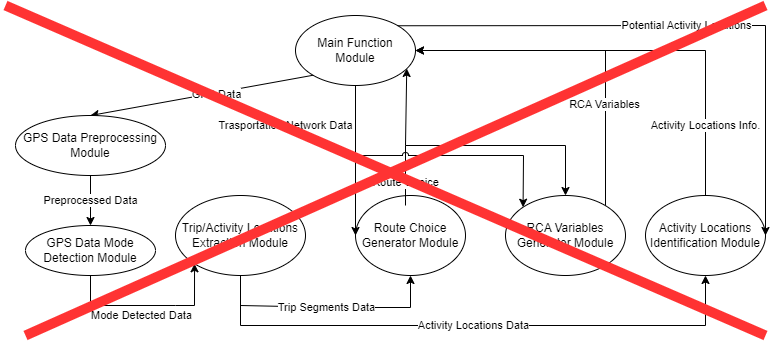
\includegraphics[scale=0.60]{Component_Diagram_old.png}
    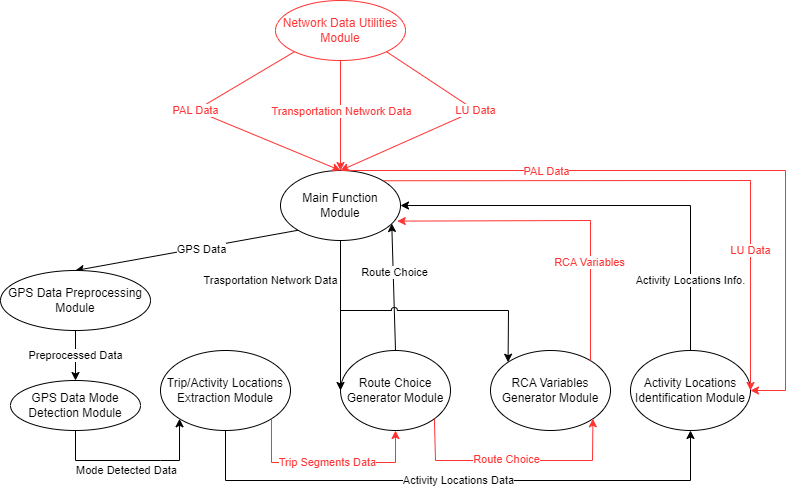
\includegraphics[scale=0.60]{Component_Diagram_new.png}
    \caption{\bf \textcolor{red}{\sout{Component Diagram} Updated Component Diagram}}
\end{figure}
\newpage

\subsection{Connection Between Requirements and Design} \label{SecConnection}
  
\subsubsection{Functional Requirements}

\begin{enumerate}
    \item Req \#1
    \begin{itemize}
        \item To satisfy this requirement, a design decision the team will implement is to use the library Pandas to read and process CSV files and use the library GeoPandas to read SHP files.
    \end{itemize}
    \item Req \#2
    \begin{itemize}
        \item To satisfy this requirement, a design decision the team will implement is to use the built-in function in GeoPandas \emph{drop\_duplicates} that will remove any duplicate points.
    \end{itemize}
    \item Req \#3
    \begin{itemize}
        \item To satisfy this requirement, a design decision the team will implement is to use GeoPandas to divide GPS points and clusters
    \end{itemize}
    \item Req \#4
    \begin{itemize}
        \item To satisfy this requirement, a design decision the team will implement is to use the given GPS input data and define a stop point (stationary) as a row that has a value of \emph{0} for the column \emph{Speed\_kmh} and the remaining rows will be trip (moving) points %\Not actually sure about this
    \end{itemize}
    \item Req \#5
    \begin{itemize}
        \item To satisfy this requirement, a design decision the team will implement is to use GeoPandas to partition GPS trajectories into segments.
    \end{itemize}
    \item Req \#6
    \begin{itemize}
        \item To satisfy this requirement, a design decision the team will implement is to sort the GPS data by segments after partitioning it and from there extract each trip segment
    \end{itemize}
    \item Req \#7
    \begin{itemize}
        \item To satisfy this requirement, a design decision the team will implement is to first define each point as a stop point or trip point. Then from there the GPS trajectories will be partitioned using GeoPandas into segments. Next, sort the GPS Data by segments. To extract the points in stop episode we simply extract the points in the stop segments. To extract the end points of trip segments we simply go to the first point in each stop segment, look at the previous point and if it is a trip point then we know that is an end point of a trip segment
    \end{itemize}
    \item Req \#8
    \begin{itemize}
        \item To satisfy this requirement, a design decision the team will implement is to use Geopandas to generate a route for any trip segment which will then generate alternative routes for entire trip segments
    \end{itemize}
    \item Req \#9
    \begin{itemize}
        \item To satisfy this requirement, a design decision the team will implement is to use GeoPandas to generate SHP files for extracted activity locations.
    \end{itemize}
    \item Req \#10
    \begin{itemize}
        \item To satisfy this requirement, a design decision the team will implement is to display an error in the command line window with a brief description as to why there is a run-time error as well as create logs using \emph{logging} to add traceability to the errors and provide a more detailed description for the error.
    \end{itemize}
    \item Req \#11
    \begin{itemize}
        \item To satisfy this requirement, a design decision the team will implement is to use GeoPandas to partition the GPS trajectories into segments. If a segment contains only stop points then it will be classified as a stop episode. If a segment contains only trip points then it will be classified as a travel episode. The team will extract each segment and put them into a separate list of GeoDataFrames, one for stop episodes and one for travel episodes. An example of what this would look like to access the first stop episode of the GPS trajectories is to define a list called \emph{stop\_episodes} and to call the first index of the list, \emph{stop\_episodes[0]}, which will output the GeoDataFrame of the first segment with only stop points, in other words, the first stop episode
    \end{itemize}
    \item Req \#12
    \begin{itemize}
        \item To satisfy this requirement, a design decision the team will implement is to use Pandas to assign values to RCA variables in CSV format.
    \end{itemize}
\end{enumerate}

\subsubsection{Look and Feel Requirements}

\begin{enumerate}
    \item LF1
    \begin{itemize}
        \item To satisfy this requirement, a design decision the team will implement is to use the command line interface to prompt the user-specific inputs and generate output files in \textcolor{red}{the} directory whose path will be displayed for the user to easily access.
    \end{itemize}
    \item LF2
    \begin{itemize}
        \item To satisfy this requirement, a design decision the team will implement is to create a progress bar on the command line as well as print out each specific stage the program is in.
    \end{itemize}
\end{enumerate}

\subsubsection{Usability and Humanity Requirements}

\begin{enumerate}
    \item UH1
    \begin{itemize}
        \item To satisfy this requirement, a design decision that will be implemented 
        is to include all of the required Python modules for the program within the same folder, which can be uploaded online as an easily downloadable zip file.
    \end{itemize}
    \item UH2
    \begin{itemize}
        \item To satisfy this requirement, a design decision that will be implemented is to include sample inputs/outputs within the program zip file, as well as provide descriptive error prompt messages when the program receives unexpected input.
    \end{itemize}
    \item UH3
    \begin{itemize}
        \item To satisfy this requirement, a design decision that will be implemented is to have a \textbf{help} flag that the user can type in the command line to display instructions on how to use the program.
    \end{itemize}
\end{enumerate}

\subsubsection{Performance Requirements}

\begin{enumerate}
    \item PR1
    \begin{itemize}
        \item To satisfy this requirement, a design decision that will be implemented is a timer function, which will output the time it took for the program to generate results after user input. This function will be used during testing.
    \end{itemize}
    \item PR2
    \begin{itemize}
        \item To satisfy this requirement, a design decision that will be implemented is a conditional statement after the user input, which will check the amount of GPS points input, and proceed with the program if there are 50 million or less GPS points in the input, or provide an error message and exit the program otherwise.
    \end{itemize}
    \item PR3
    \begin{itemize}
        \item To satisfy this requirement, a design decision that will be implemented is to avoid using any time-sensitive packages or libraries within the program.
    \end{itemize}
\end{enumerate}

\subsubsection{Operational and Environmental Requirements}

\begin{enumerate}
    \item OE1
    \begin{itemize}
        \item To satisfy this requirement, a design decision that will be implemented is to avoid using any libraries, packages, or code within the program that are restricted by an operating system.
    \end{itemize}
    \item OE2
    \begin{itemize}
        \item To satisfy this requirement, a design decision that will be implemented is to avoid using any external packages within the code, and only use open-source Python packages.
    \end{itemize}
    \item OE3
    \begin{itemize}
        \item To satisfy this requirement, a design decision that will be implemented is to include all of the required Python packages within a 'requirements.txt' text file. These packages will be able to be installed using 'pip install -r requirements.txt'.
    \end{itemize}
\end{enumerate}

\subsubsection{Maintainability and Support Requirements}

\begin{enumerate}
    \item MS1
    \begin{itemize}
        \item To satisfy this requirement, a design decision that will be implemented is to have all of the source code for the program located on a GitHub repository, which will be modified any time there are changes to the program.
    \end{itemize}
    \item MS2
    \begin{itemize}
        \item To satisfy this requirement, a design decision that will be implemented is that the GitHub repository the program is located on will have an option for developers to open tickets.
    \end{itemize}
    \item MS3
    \begin{itemize}
        \item To satisfy this requirement, a design decision that will be implemented is to avoid using any packages, libraries, or code that depend on the user's current location within the program.
    \end{itemize}
\end{enumerate}

\subsubsection{Security Requirements}

\begin{enumerate}
    \item SR1
    \begin{itemize}
        \item To satisfy this requirement, a design decision that will be implemented is to avoid using any packages, libraries, or code that stores the user's personal information.
    \end{itemize}
    \item SR2
    \begin{itemize}
        \item To satisfy this requirement, a design decision that will be implemented is to avoid using any packages, libraries, or code that uses files outside of the user-provided inputs and files included in Python and the program directory.
    \end{itemize}
    \item SR3
    \begin{itemize}
        \item To satisfy this requirement, a design decision that will be implemented is to push a Git commit with a descriptive message whenever a meaningful change is made to the source code.
    \end{itemize}
\end{enumerate}

\subsubsection{Legal Requirements}

\begin{enumerate}
    \item LR1
    \begin{itemize}
        \item To satisfy this requirement, a design decision the team will implement is to use free-use open-source packages such as GeoPandas for the development of the product.
    \end{itemize}
\end{enumerate}

\section{System Variables}
N/A
% \wss{Include this section for Mechatronics projects}

% \subsection{Monitored Variables}

% \subsection{Controlled Variables}

% \subsection{Constants Variables}

\section{User Interfaces}
The product is designed to interact with the user through command-line prompts, which is the same as the existing implementation of GERT. Examples of the user interface can be found in Appendix \ref{UI}.
As stated in the \href{https://github.com/paezha/PyERT-BLACK/blob/main/docs/ProblemStatementAndGoals/ProblemStatement.pdf}{Problem Statement and Goals} \citep{ProblemStatement} document, implementing the GUI would be considered a stretch goal for the current version of the system.


% \wss{Design of user interface for software and hardware.  Attach an appendix if
% needed. Drawings, Sketches, Figma}

\section{Design of Hardware}
N/A

% \wss{Most relevant for mechatronics projects}
% \wss{Show what will be acquired}
% \wss{Show what will be built, with detail on fabrication and materials}
% \wss{Include appendices as appropriate, possibly with sketches, drawings, CAD, etc}

\section{Design of Electrical Components}
N/A

% \wss{Most relevant for mechatronics projects}
% \wss{Show what will be acquired}
% \wss{Show what will be built, with detail on fabrication and materials}
% \wss{Include appendices as appropriate, possibly with sketches, drawings,
% circuit diagrams, etc}

\section{Design of Communication Protocols}
N/A
% \wss{If appropriate}

\newpage
\section{Timeline}
\begin{table}[h!]
    \centering
    \begin{tabular}{|>{\raggedright}p{0.2\textwidth}|p{0.4\textwidth}|p{0.125\textwidth}|p{0.2\textwidth}|}
    \hline
    \textbf{Modules} & \textbf{Rev 0 Implementation Tasks} & \textbf{Deadline} & \textbf{Team Members Responsible}\\
    \hline
     Hardware-Hiding Module & Provided by OS & N/A & N/A\\
    \hline
     GPS Data Preprocessing Module & Implement all the functions included in the module & \textcolor{red}{\sout{February 6} January 27}, 2023 & Jasper, Mike\\
    \hline
     GPS Data Mode Detection Module & Implement all the functions included in the module & February \textcolor{red}{\sout{6} 4}, 2023 & Jasper, Mike\\
    \hline
     Trip Segments and Activity Locations Extraction Module & Implement all the functions included in the module & February \textcolor{red}{\sout{6} 9}, 2023 & Jasper, Mike\\
    \hline
     Route Choice Set Generator Module & Implement all the functions included in the module & \textcolor{red}{\sout{February 6} January 27}, 2023 & Mengtong, Hongzhao\\
    \hline
     Route Choice Analysis Variables Generator Module & Implement all the functions included in the module & February \textcolor{red}{\sout{6} 4}, 2023 & Linqi, Hongzhao\\
    \hline
     Activity Locations Identification Module & Implement all the functions included in the module & February \textcolor{red}{\sout{6} 9}, 2023 & Zabrain\\
    \hline
     Main Function Module & Implement all the functions included in the module & February \textcolor{red}{\sout{6} 14}, 2023 & All team members\\
    \hline
     Dataframe Data Structure Module & Provided by external libraries & N/A & N/A\\
    \hline
     GeoDataframe Data Structure Module & Provided by external libraries & N/A & N/A\\
    \hline
     OSM Network Dataset Reader Module & Provided by external libraries & N/A & N/A\\
    \hline
     Plotting Module & Provided by external libraries & N/A & N/A\\
    \hline
    \end{tabular}
    \caption{Timeline \textcolor{red}{for Rev 0 Implementation}}
    \label{tab:timeline}
\end{table}

\begin{table}[h!]
    \color{red}
    \centering
    \begin{tabular}{|>{\raggedright}p{0.2\textwidth}|p{0.4\textwidth}|p{0.125\textwidth}|p{0.2\textwidth}|}
    \hline
    \textbf{Modules} & \textbf{Unit Tests Tasks} & \textbf{Deadline} & \textbf{Team Members Responsible}\\
    \hline
     Hardware-Hiding Module & Provided by OS & N/A & N/A\\
    \hline
     GPS Data Preprocessing Module & Test all the functions included in the module & March 1, 2023 & Jasper, Mike\\
    \hline
     GPS Data Mode Detection Module & Test all the functions included in the module & March 2, 2023 & Jasper, Mike\\
    \hline
     Trip Segments and Activity Locations Extraction Module & Test all the functions included in the module & March 3, 2023 & Jasper, Mike\\
    \hline
     Route Choice Set Generator Module & Test all the functions included in the module & March 1, 2023 & Mengtong, Hongzhao\\
    \hline
     Route Choice Analysis Variables Generator Module & Test all the functions included in the module & March 2, 2023 & Linqi, Hongzhao\\
    \hline
     Activity Locations Identification Module & Test all the functions included in the module & March 3, 2023 & Zabrain\\
    \hline
     Main Function Module & Test all the functions included in the module & March 4, 2023 & All team members\\
    \hline
     Dataframe Data Structure Module & Provided by external libraries & N/A & N/A\\
    \hline
     GeoDataframe Data Structure Module & Provided by external libraries & N/A & N/A\\
    \hline
     OSM Network Dataset Reader Module & Provided by external libraries & N/A & N/A\\
    \hline
     Plotting Module & Provided by external libraries & N/A & N/A\\
    \hline
    \end{tabular}
    \caption{Timeline for Unit Tests}
    \label{tab:timeline}
\end{table}

% \wss{Schedule of tasks and who is responsible}
The \textcolor{red}{updated} Gantt Chart of the project timeline can be found \href{https://github.com/paezha/PyERT-BLACK/blob/main/docs/Project%20Schedule/Capstone%20timeline.pdf}{here}.

% \bibliographystyle {plainnat}
% \bibliography{../../../refs/References}
\bibliographystyle{plainnat}

% \bibliography{../../refs/References}
\bibliography{SystDes}

\newpage{}

\appendix

\section{Interface}
\label{UI}
% \wss{Include additional information related to the appearance of, and
% interaction with, the user interface}
The system will ask for user inputs through command-line prompts as shown in Figure \ref{fig:input}.
\begin{figure}[H]
    \centering
    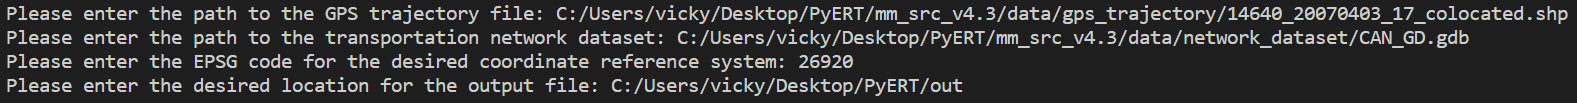
\includegraphics[scale=0.55]{input.png}
    \caption{\bf Input}
    \label{fig:input}
\end{figure}

The system will tell the user which stage it is in as shown in Figure \ref{fig:stages}.
\begin{figure}[H]
    \centering
    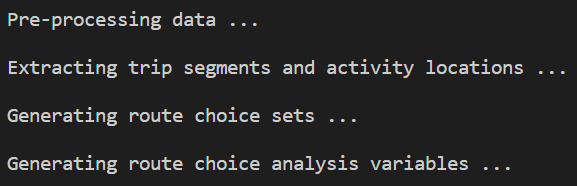
\includegraphics[scale=0.55]{stages.png}
    \caption{\bf Stages}
    \label{fig:stages}
\end{figure}

The system will show the user where the output files are and display the URL to the generated map as illustrated in Figure \ref{fig:output}.
\begin{figure}[H]
    \centering
    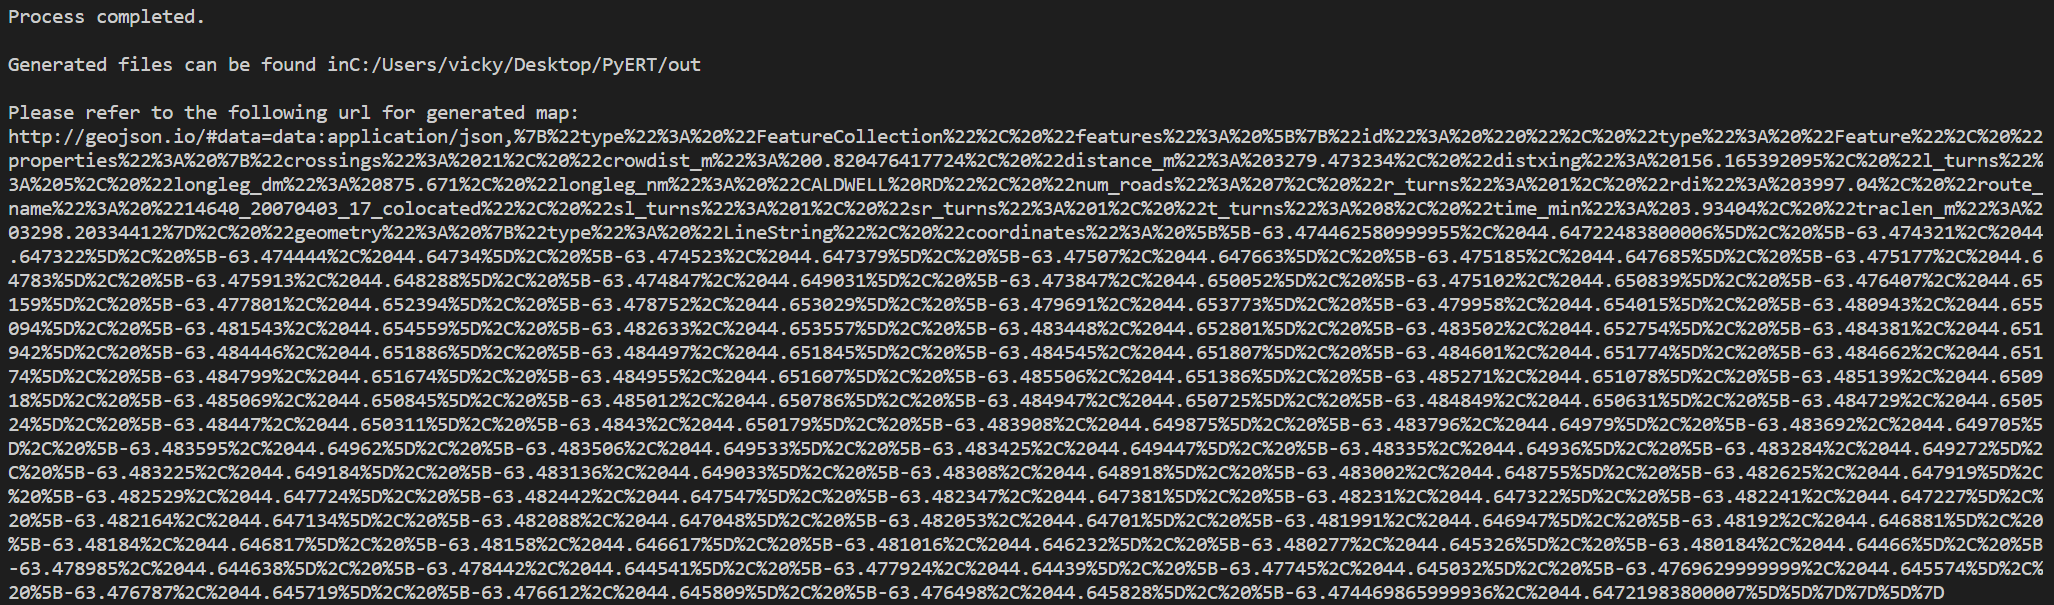
\includegraphics[scale=0.4]{output.png}
    \caption{\bf Output}
    \label{fig:output}
\end{figure}

The system will tell the user when an error occurs through error and warning messages, as shown in Figure \ref{fig:error} and \ref{fig:warning}, respectively.
\begin{figure}[H]
    \centering
    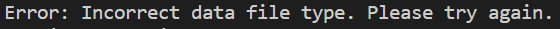
\includegraphics[scale=0.55]{error.png}
    \caption{\bf Error Message}
    \label{fig:error}
\end{figure}

\begin{figure}[H]
    \centering
    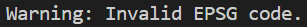
\includegraphics[scale=0.55]{warning.png}
    \caption{\bf Warning Message}
    \label{fig:warning}
\end{figure}

\section{Mechanical Hardware}
N/A

\section{Electrical Components}
N/A

\section{Communication Protocols}
N/A

\section{Reflection}

The information in this section will be used to evaluate the team members on the
graduate attribute of Problem Analysis and Design.  Please answer the following questions:

\begin{enumerate}
  \item What are the limitations of your solution?  Put another way, given
  unlimited resources, what could you do to make the project better? (LO\_ProbSolutions)
  \\
  \\
  One limitation of our solution is that it does not provide all of the same functionality as GERT. GERT provides an option to input Time Use Diaries (data sets which tracks person's activities throughout the day), and use those to create additional outputs. Since we were not able to obtain samples of what these Time Use Diaries, and also were limited by time, we were unable to implement this feature. If given unlimited time and resources, we would implement additional modules to process these diaries and generate additional outputs.
  \\
  \\
  Another limitation of our solution is that it does not have a GUI. The current proposed implementation will run using the command line. This is not as intuitive as a GUI, especially for the target audience of geography researchers/students who may not have experience with Python or the command line. If given unlimited resources and time, we would have created a Python application, which would not require any running of commands, and the user would be able to drag and drop inputs into the application window.
  
  
  \item Give a brief overview of other design solutions you considered.  What
  are the benefits and tradeoffs of those other designs compared with the chosen
  design?  From all the potential options, why did you select documented design? (LO\_Explores)
  \\
  \\
  One design solution we considered was to copy the design of the original GERT project, but replace all of the function calls which used the ArcPy package (a python package for ArcGIS, which required the ArcGIS License to be used) with our own code. The proposed plan was to use the ArcPy documentation and recreate all of the functions with GeoPandas/ similar python packages. The benefit of doing this would be that we wouldn't have to worry about designing our own software architecture, since we could just re-use the architecture from the original working GERT project. Also, replacing all of the code would ensure that our solution would provide the same functions as GERT. However, the tradeoff was that learning about and re-implementing the different functions provided by ArcPy would be too time consuming, compared to finding our own way to process the data.


\end{enumerate}

\end{document}